% !TeX spellcheck = en_GB
\begin{figure}[t!]
	\centering
	\begin{subfigure}[b]{0.49\textwidth}
		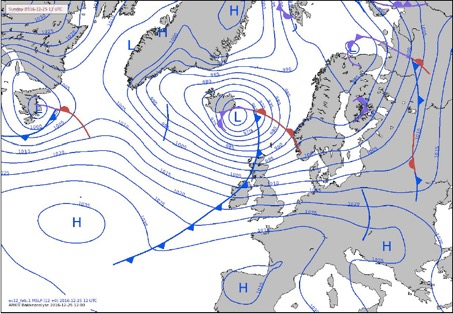
\includegraphics[width=\textwidth]{./fig_introduction/Ana_2512_12UTC.jpg}
		\caption{}\label{fig:ana_YR}
	\end{subfigure}
	\hfill
	\begin{subfigure}[b]{0.49\textwidth}
		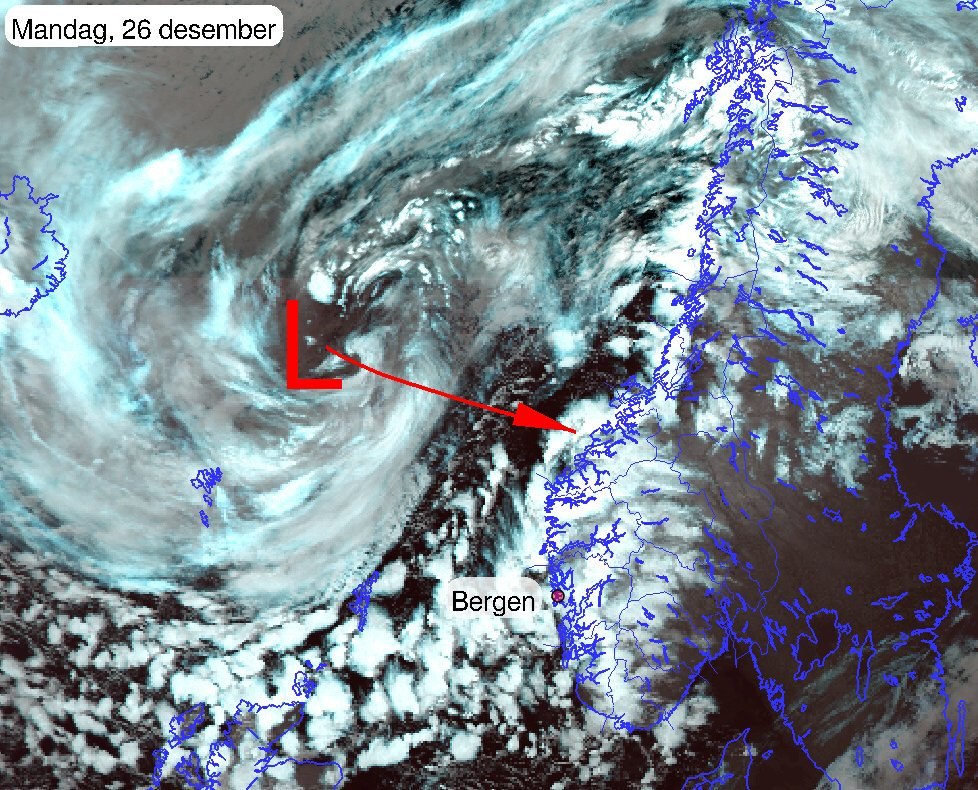
\includegraphics[trim={0cm 3.8cm 0cm 0cm},clip, width=\textwidth]{./fig_introduction/Twitter_26122016_0934AM.jpeg}
		\caption{}\label{fig:meteorologene_2612}	
	\end{subfigure}
	\begin{subfigure}[b]{0.49\textwidth}
		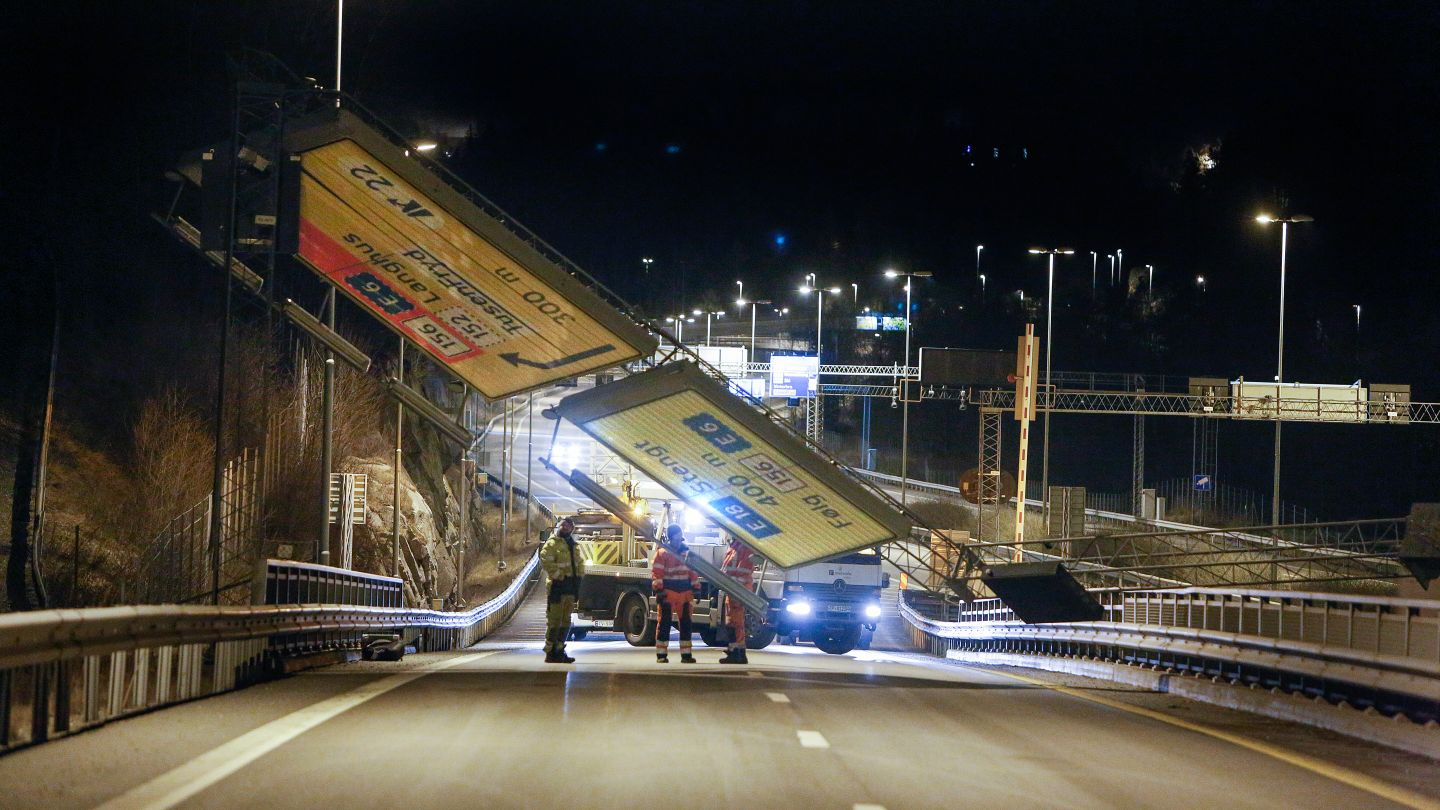
\includegraphics[width=\textwidth]{./fig_introduction/street_sign_2512.jpg}
		\caption{}\label{fig:street_sign}
	\end{subfigure}
	\hfill
	\begin{subfigure}[b]{0.49\textwidth}
		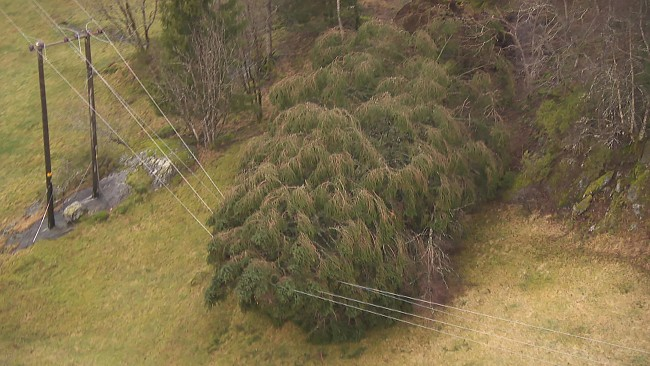
\includegraphics[width=\textwidth]{./fig_introduction/tree_nrk_2812.jpg}
		\caption{}\label{fig:tree_elec}
	\end{subfigure}
	\caption{Weather situation during the extreme Christmas storm and impact on the infrastructure. \protect\subref{fig:ana_YR}: Weather situation Sunday \SI{25}{\dec} at \SI{12}{\UTC} from 
		%the extreme weather report on Urd 
		\citep{olsen_ekstremvaerrapport._2017}.
		\protect\subref{fig:meteorologene_2612}: Tweet from \cite{meteorologene_her_2016} on \SI{26}{\dec} at 9:34 am. %: Here comes \#Urd! The low pressure centre will hit M{\o}re og Romsdal, but the strongest wind comes south of Stad. \#S{\o}rNorge.
		\protect\subref{fig:street_sign} and \protect\subref{fig:tree_elec}: %show the 
		Consequences related to the high wind speeds during Christmas 2016 \citep{ruud_tonn_2016,farestveit_80.000_2016}.
		%\protect\subref{fig:street_sign}: This traffic sign, ten meter long and four meter high was blown over during the storm, .
		%\protect\subref{fig:tree_elec}: Trouble maker: The extreme weather during Christmas created problems for the local infrastructure. \num{80.000} households were without electricity during the storm, \citep{}.
	} \label{fig:news}
\end{figure}